\documentclass[10pt, compress]{beamer}

\usetheme{m}

\usepackage{booktabs}
\usepackage[scale=2]{ccicons}
\usepackage{minted}

\usepackage{graphicx} %package to manage images


\usepackage{tikz}

\usetikzlibrary{scopes}
%\documentclass[tikz, border=5pt]{standalone}
\usetikzlibrary{calc}
\usetikzlibrary{patterns}
\usepackage{tkz-euclide}
\usetkzobj{all}

\usemintedstyle{trac}

\usefonttheme[onlymath]{serif}

\newcommand\der{{\rm d}}

\title{Robot Inverse Kinematics using SQP method}
\subtitle{}
\date{\today}
\author{Xiaoqian Mu, Yuechuan Xue}
\institute{Iowa State University}

\begin{document}

\maketitle

\begin{frame}[fragile]{Problem Formulation}
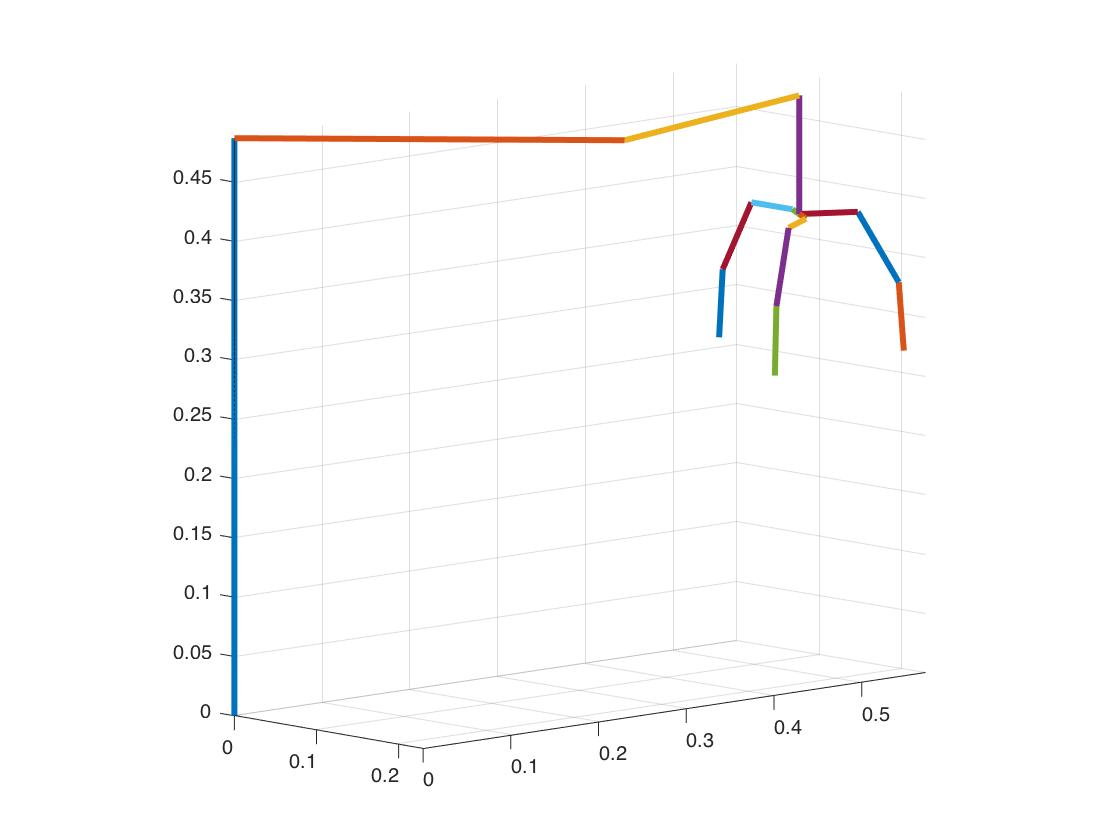
\includegraphics[width=6cm, height=4cm]{robot-matlab-config.jpg}
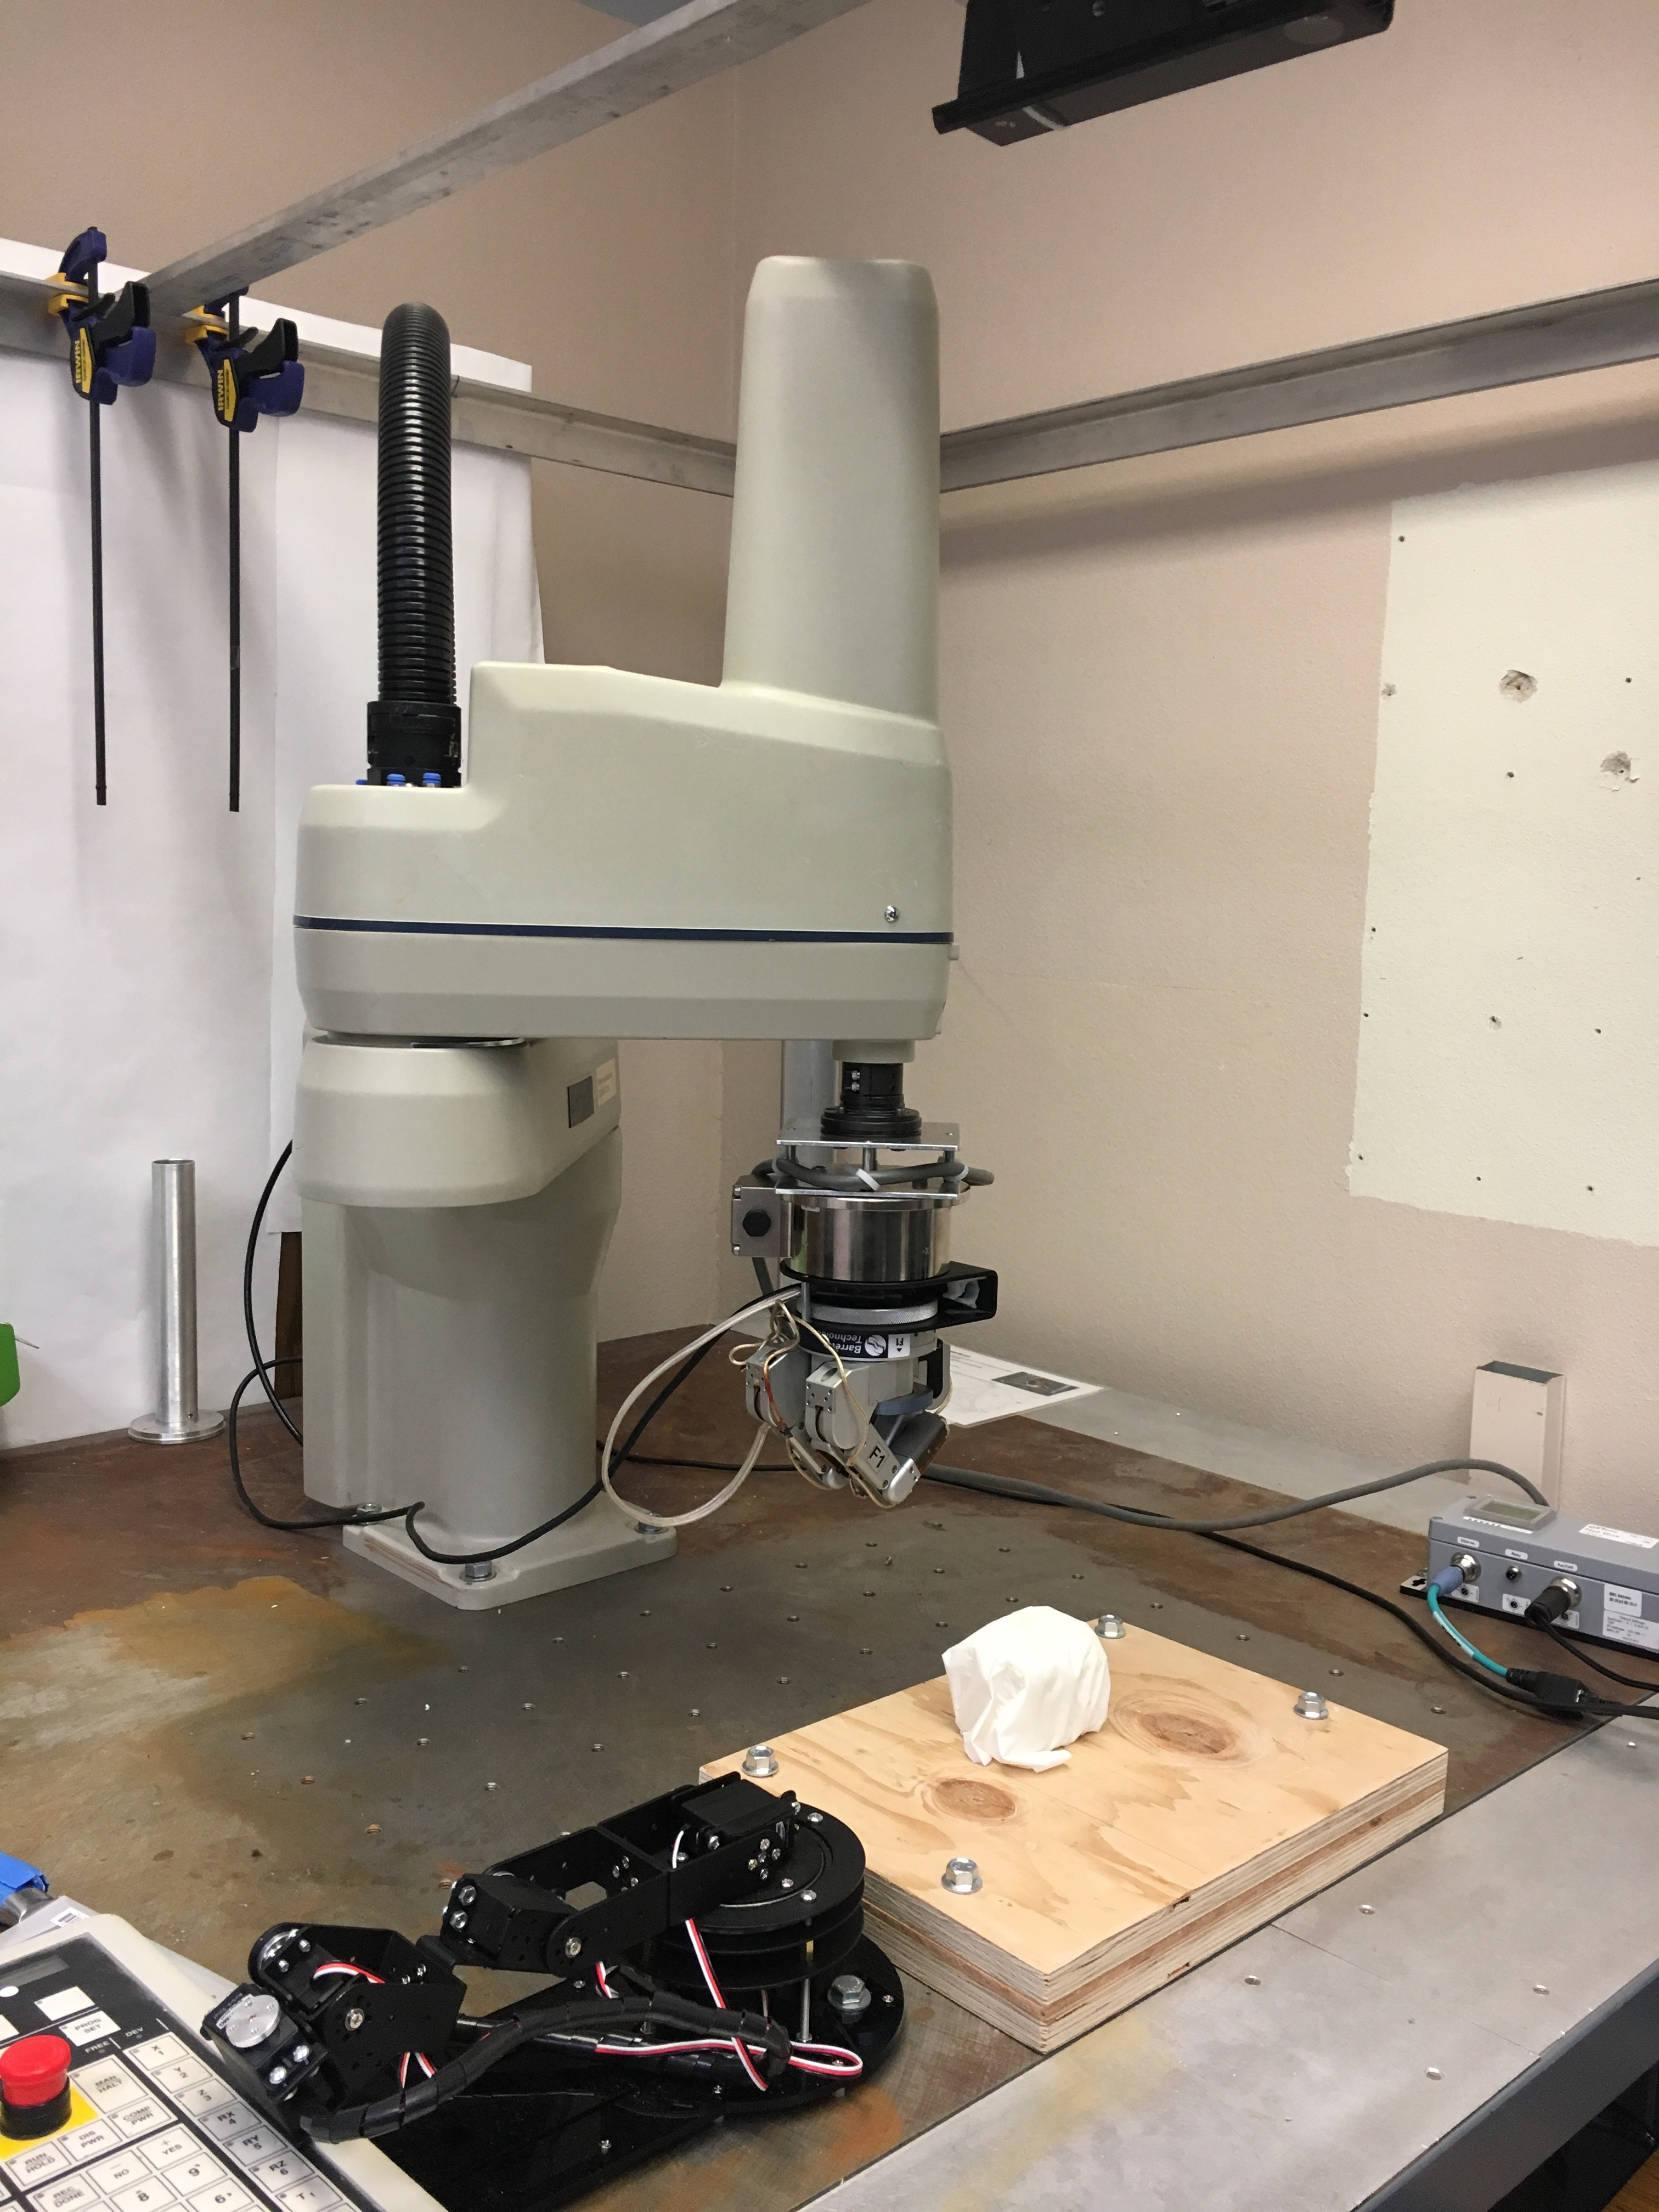
\includegraphics[width=4cm, height=5cm]{IMG_5860.jpg}
\end{frame}



\begin{frame}[fragile]{Introduction}
\begin{columns}
\begin{column}{0.5\textwidth}
In constrained optimization, the general aim is to transform the problem into an easier subproblem that can then be solved and used as the basis of an iterative process.

\vspace{0.1in}

Some early methods translate the constrained problem to a basic unconstrained problem by using a \textbf{penalty function} for constraints  that are near or beyond the constraint boundary. (Interior Point Method)
\end{column}
\begin{column}{0.5\textwidth}  %%<--- here
    \begin{center}
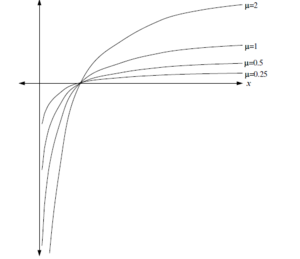
\includegraphics[width=4cm, height=5cm]{interior-point-method.png}
     \end{center}
\end{column}
\end{columns}
\end{frame}

\begin{frame}[fragile]{Introduction}
These methods are now considered relatively inefficient and have been replaced by methods that have focused on the solution of the KKT equations.

The KKT are necessary conditions for optimality for a constrained optimization problem. It is both necessary and sufficient for a global optimal point in a convex programming problem. 
\end{frame}

\begin{frame}[fragile]{Sequential Quadratic Programming}
A series of algorithms attempt to compute the Lagrange multipliers directly.

Constrained quasi-Newton methods guarantee super-linear convergence by accumulating second-order information regarding the KKT equations using a quasi-Newton updating procedure.

A quadratic programming (QP) problem will be solved at each major iteration.
\end{frame}

\begin{frame}[fragile]{Sequential Quadratic Programming}
Principal idea: \textbf{Formulate a QP subproblem based on a quadratic approximation of the Lagrangian function.}
$$L(x, \lambda) = f(x) + \sum_{i=1}^m \lambda_i \cdot g_i(x)$$

At each major iteration, an approximation is made of the Hessian of Lagrangian function. The constraints are approximated linearly. 

The solution of QP subproblem will be used to form a search direction for a line search procedure.
\end{frame}

\begin{frame}[fragile]{Sequential Quadratic Programming}
QP SubProblem:
$$ \min {1 \over 2} d^\top H_k d + \nabla f(x_k)^\top d$$
\begin{eqnarray*}
	\nabla g_i(x_k)^\top d + g_i(x_k) & = & 0, i = 1,\cdots, m_e \\
	\nabla g_i(x_k)^\top d + g_i(x_k) & \leq & 0, i = m_e+1,\cdots, m
\end{eqnarray*}
\end{frame}

\begin{frame}[fragile]{Sequential Quadratic Programming}
The SQP implementation consists of three main stages:
\begin{itemize}
  \item Updating the Hessian Matrix
  \item Quadratic Programming Solution
  \item Line Search and Merit Function
\end{itemize}
\end{frame}

\begin{frame}[fragile]{Updating the Hessian Matrix}
At each major iteration, a positive definite quasi-Newton approximation of the Hessian of Lagrangian function, $H$, is calculated using the \textbf{BFGS} method, where $\lambda_i, i = 1\cdots m$, is an estimate of the Lagrange
$$C_k^{\rm BFGS} = {q_kq_k^\top \over q_k^T s_k} - {H_k p_k p_k^\top H_k^\top \over p_k^\top H_k p_k}$$
$$H_{k+1} = H_{k} + C_k^{\rm BFGS}$$
\end{frame}

\begin{frame}[fragile]{Quadratic Programming Solution}
At each major iteraion, a QP problem of the following form is solved
$$\min {1 \over 2} d^\top H_k d + c^\top d$$
\begin{eqnarray*}
A_i d = b_i, \quad i = 1,\cdots , m_e \\
A_i d = b_i, \quad i \leq m_e + 1,\cdots , m
\end{eqnarray*}
\end{frame}

\begin{frame}[fragile]{Line Search and Merit Function}
The solution to the QP subproblem produces a vector $d_k$, which is used to form a new iterate
$$\boldsymbol{x}_{k+1} = \boldsymbol{x}_k + \alpha \boldsymbol{d}_k$$
The step length parameter $\alpha_k$ is determined in order to produce a sufficient decrease in a \textbf{merit function}. 

Merit Function:
$$\Psi = f(x) + \sum_{i = 1}^{m_e} r_i \cdot g_i(x) + \sum_{i = m_e + 1}^{m} r_i \cdot \max [0, g_i(x)]$$
where $r_i$ is a penalty parameter.
\end{frame}

\end{document}